\chapter{Implementation and Tests}

This chapter provides a practical overview of the proposed integrity
verification protocol by presenting a real implementation developed specifically for this work. The implementation consists of a standalone binary application built around the \texttt{mt-rs} library, employing the BLAKE3 cryptographic hash function, the Raft consensus algorithm, and the Reed-Solomon coding.

Rather than including extensive code listings, which would not significantly contribute to the goals of this thesis, the discussion highlights selected code snippets that illustrate how the individual components operate together in a coherent system. Finally, the chapter presents a series of benchmarks designed to evaluate the behavior of the implementation under various scenarios, such as node failures, varying numbers of agents, and datasets of different sizes and file counts.

\section{Files in a Raft Cluster}

As discussed in Section \ref{sec:raft-cluster-for-file-uploads}, the system is built upon a Raft cluster integrated with a storage mechanism based on Reed-Solomon codes. To study this integration, a Go\footnote{\url{https://go.dev/}} application was implemented, reconstructing a Cubbit-like infrastructure by layering a Raft cluster on top of Reed-Solomon redundancy. Go was chosen for its gentle learning curve and widespread adoption, including by companies such as Cubbit. Following the common project layout recommended for Go\cite{go-modules-layout} all the developed services are organized within a single module. This structure avoids redundancy, such as duplicating the service message definitions described later. Each service is maintained separately as a distinct binary under the \texttt{cmd/} folder, in accordance with Go best practices.



To investigate communication patterns between the system components, two service APIs were implemented: a REST API, widely used for web services, and gRPC\footnote{\url{https://grpc.io/}}, developed by Google and based on Protobuf, which allows precise definition of the message types transmitted over the network.

\begin{listing}[H]
\caption{Protobuf definitions for the \texttt{Agent} service, used for communication between gateways and agents, as well as among agents themselves. The file is located in \texttt{internal/proto/agent.proto}.}
\label{code:protobuf-for-agent}
\begin{minted}[linenos,fontsize=\footnotesize]{protobuf}
service Agent {
    rpc SendShard(ShardRequest) returns (ShardResponse) {}
    rpc GetShard(ShardGetRequest) returns (ShardGetResponse) {}
    rpc AckShard(ShardAckRequest) returns (ShardAckResponse) {}
    rpc GetRootHash(RootHashRequest) returns (RootHashResponse) {}
    rpc JoinRaft(JoinRequest) returns (JoinResponse) {}
}

message ShardRequest {
    string filename = 1;
    int64 index = 2;
    bytes data = 3;
}

message ShardGetRequest {
    string filename = 1;
    int64 index = 2;
}

message ShardAckRequest {
    string filename = 1;
    int64 index = 2;
    bytes roots = 3;
}

message ShardResponse {
    string filename = 1;
    bytes salt = 2;
}

message ShardGetResponse { bytes data = 1; }

message ShardAckResponse { bool status = 1; }

message RootHashRequest { bytes folder = 1; }

message RootHashResponse { bytes hash = 1; }

// ...
\end{minted}
\end{listing}

Listing \ref{code:protobuf-for-agent} illustrates the Protobuf definitions used by the agents, including messages for both gateway-agent and agent-agent interactions.

The distinctive feature of gRPC is that the Protobuf file can be directly compiled into Go code using a simple CLI, as shown in Listing \ref{code:protobuf-protoc}.

\begin{listing}
\caption{Protobuf compiler command that generates Go code from the service definition located at \texttt{agent.proto}.}
\label{code:protobuf-protoc}
\begin{minted}{shell}
protoc --go_out=. \
        --go_opt=paths=source_relative \
        --go-grpc_out=. \
        --go-grpc_opt=paths=source_relative \
        agent.proto
\end{minted}
\end{listing}

This command generates two Go files: 
\begin{itemize}
    \item \texttt{agent.pb.go}, which contains the standard Protobuf message definitions and serialization code.
    \item \texttt{agent\_grpc.pb.go}, which contains the gRPC client and server stubs necessary to implement the service endpoints in Go. The methods defined in Listing \ref{code:protobuf-for-agent} are represented as an interface in this file, and they must be implemented to enable communication between a gateway and the agent service, or among agents themselves.
\end{itemize}

Together, these files constitute the foundation for both gateway-to-agent and inter-agent communication in the system.

\subsection{Gateway service} 

The Gateway acts as the entry point for the user, as illustrated in step 1 of Figure \ref{fig:sequence-diagram-upload-file}. It is exposed via a REST API and manages file uploads and downloads by splitting files into $n+k$ shards using the Reed-Solomon algorithm and distributing them across the agents. The REST interface is intentionally minimal in this prototype, offering only two endpoints: one for uploading and one for downloading files. The upload endpoint requires the local file path and the desired filename, while the download endpoint requires only the filename.

Go provides a straightforward mechanism to instantiate a web server, as shown in Listing \ref{code:mux-gateway}. The \texttt{mux} server maps REST paths to functions, referred to as handlers. 

\begin{listing}\caption{Instantiation of a simple web server in Go.}

\label{code:mux-gateway}
\begin{minted}[linenos,fontsize=\footnotesize]{go}
mux := &http.ServeMux{}
mux.HandleFunc("/upload", UploadHandler)
mux.HandleFunc("/download/{filename}", DownloadHandler)
http.ListenAndServe("<url>", mux);
\end{minted}
\end{listing}


\paragraph{Upload handler}

A partial implementation of the upload handler is shown in Listing \ref{code:upload-handler}.

\begin{listing}
\caption{Upload handler: Gateway orchestrates file encryption, Reed-Solomon shard creation, and transmission to agents via the \texttt{rpc.SendShard} wrapper.}
\label{code:upload-handler}
\begin{minted}[linenos,fontsize=\footnotesize]{go}
func UploadHandler(w http.ResponseWriter, r *http.Request) {
    // Open the file in byte format.
    // Generate a key and encrypt the file with it.
    // Encrypt the local file using a random key.
    ciphertext, err := cryptography.Enc(file, key)
    
    // Create N+K shards from the encrypted file ([][]byte).
    shardBytes, err := reedSolomon.Create(N, K, ciphertext)

    // Generate a "good" salt to extend the filename.
    // Send each shard to a different agent.
    for i, shard := range shardBytes {
        resp, err := rpc.SendShard(
            cfg.Agents[i], filename+salt, i, shard,
        )

        if err != nil {
            // Handle error
        }
    }
    
    // Build a JSON response for the client.
    jsonResponse, _ := json.Marshal(/* ... */)

    w.Header().Set("Content-Type", "application/json")
    w.Write(jsonResponse)
}

\end{minted}
\end{listing}

Some clarifications on the code in Listing \ref{code:upload-handler} are in order.
The details of file encryption are omitted, since they are not central to the current discussion. Similarly, the internal implementation of Reed-Solomon encoding is abstracted: the key point is that the function \texttt{reedSolomon.Create} returns the $n+k$ shards from the encrypted file. Error handling is also simplified for readability, and the specific contents of the \texttt{jsonResponse} are not reported, as they are not relevant to the design.

The critical part lies in lines 14-16, where the \texttt{SendShard} method from the custom \texttt{rpc} module is invoked. This method serves as a wrapper around the generated gRPC client code contained in \texttt{agent\_grpc.pb.go}. Its role is to establish the connection, transmit the shard, and delegate the call to the gRPC stub. The implementation of this wrapper is presented in Listing \ref{code:rpc-send-shard}.

However, this implementation alone is not sufficient. A corresponding gRPC server must also be defined to handle the data transmitted in lines 27-31. As explained earlier, the code in \texttt{agent\_grpc.pb.go} only provides the interface definition; the concrete server-side logic needs to be implemented in order to process the incoming shard data. This aspect will be discussed in detail in the next section.

\begin{listing}
\caption{\texttt{SendShard} wrapper: intermediate function that establishes a gRPC connection to the target Agent, forwards the shard data to the generated gRPC client stub in \texttt{agent\_grpc.pb.go}, and returns the response.}
\label{code:rpc-send-shard}
\begin{minted}[linenos,fontsize=\footnotesize]{go}
func SendShard(agent, filename string, index int, 
    data []byte) (*pb.ShardResponse, error) {
    dialCtx, dialCancel := 
        context.WithTimeout(context.Background(), 100*time.Millisecond)
	defer dialCancel()

    conn, _ := grpc.DialContext(dialCtx, agent,
            grpc.WithTransportCredentials(insecure.NewCredentials()),
            grpc.WithBlock())
    defer conn.Close()

    // Instantiate the gRPC client for the Agent service.
    c := pb.NewAgentClient(conn) 

    ctx, cancel := context.WithTimeout(context.Background(), time.Second)
    defer cancel()

    // Call the SendShard procedure for the i-th shard of the file.
    resp, _ := c.SendShard(ctx, &pb.ShardRequest{
        Filename: filename, Index: int64(index), Data: data,
    })

    return resp, nil
}
\end{minted}
\end{listing}

\paragraph{Download handler}

Equally important, though similar in structure to the previously presented \texttt{UploadHandler}, is the \texttt{DownloadHandler}. While not strictly necessary for system testing, it is useful in both real-world scenarios and tests, for example to verify that a downloaded file is not corrupted. A partial implementation is shown in Listing \ref{code:download-handler}.

\begin{listing}
\caption{Download handler: logic that retrieves all shards of a file via the \texttt{rpc.GetAllShards} wrapper, reconstructs the file using Reed-Solomon, decrypts it, and returns it as a download to the user.}
\label{code:download-handler}
\begin{minted}[linenos,fontsize=\footnotesize]{go}
func DownloadHandler(w http.ResponseWriter, r *http.Request) {
    // Retrieve the salt for a given filename 
    // to reconstruct the exact file saved on agents.
    endFile := getEndFile(filename, salt)

    // Retrieve all shards from agents
    shards, _ := rpc.GetAllShards(endFile)

    // Reconstruct the entire file using Reed-Solomon,
    // and store it at endFile path
    _ = reedSolomon.Reconstruct(cfg.N, cfg.K, endFile, shards)
    // Decrypt the reconstructed file and store it as filename

    // Return the plaintext file as an attachment
    w.Header()
        .Set("Content-Disposition",
            fmt.Sprintf("attachment; filename=%s", filename),
        )
    content, _ = ioutil.ReadFile(filename)

    // Handle possible errors and clear temporary files

    w.Write(content)
}
\end{minted}
\end{listing}

As with the \texttt{UploadHandler}, certain implementation details are omitted for simplicity, such as how the correct salt is determined for each file and the internal workings of the Reed-Solomon reconstruction algorithm. The \texttt{rpc.GetAllShards} function serves as a wrapper, analogous to \texttt{SendShard} in Listing \ref{code:rpc-send-shard}. Internally, it executes gRPC calls to the \texttt{GetShard} method defined in the Protobuf file (Listing \ref{code:protobuf-for-agent}), the server-side handling of which will be discussed in the following section.

\newpage

\subsection{Agent service}

Each agent is responsible for storing its assigned shards locally and participates as a node in the Raft cluster. The total number of agents corresponds to the Reed-Solomon configuration $n+k$. Communication between the gateway and agents is implemented using gRPC, which enables efficient binary data transfer and supports a wide range of commands. Inter-agent communication also relies on gRPC, providing operations such as shard acknowledgments, cluster membership management, and retrieval of the current Merkle root hash for a given folder.

\paragraph{Instance new agent}

The Agent service must instantiate a new gRPC server at startup, while also initializing its participation in the Raft cluster. When a node starts a new cluster, the process is referred to as \emph{bootstrapping}. A simplified version of the Agent service startup is shown in Listing \ref{code:agent-main-go}.

\begin{listing}[H]
\caption{Agent service startup. The gRPC server is initialized and registered, and the node joins or bootstraps a Raft cluster.}
\label{code:agent-main-go}
\begin{minted}[linenos,fontsize=\footnotesize]{go}
import (
    pb "<path_with_proto_files>"
    // ...
)

// Server implements the gRPC service defined in the Protobuf file.
type Server struct {
    pb.UnimplementedAgentServer
    RaftServer *raft.Server
    // Other fields
}

s := grpc.NewServer()
reflection.Register(s)
server := server.Server{}

// Register the gRPC server with the generated Protobuf bindings.
pb.RegisterAgentServer(s, &server)

server.RaftServer = newRaft(ctx, ..., ..., ..., ...)

lis, _ := net.Listen("tcp", uri)
s.Serve(lis)
\end{minted}
\end{listing}

Some details are omitted in Listing \ref{code:agent-main-go}, such as error handling, but two elements are particularly important:
the \texttt{Server} struct, which implements the service interface generated from the Protobuf definition, and the \texttt{newRaft} function, which initializes a new Raft instance.  

For this prototype, the HashiCorp Raft implementation\footnote{\url{https://github.com/hashicorp/raft}} has been adopted. A partial implementation of \texttt{newRaft} is shown in Listing \ref{code:new-raft-function}.

\begin{listing}[H]
\caption{Partial implementation of the \texttt{newRaft} function, which initializes the Raft consensus node.}
\label{code:new-raft-function}
\begin{minted}[linenos,fontsize=\footnotesize]{go}
import (
    "github.com/hashicorp/raft"
    boltdb "github.com/hashicorp/raft-boltdb"
    // ...
)

func newRaft(ctx context.Context, bootstrap bool, id, raftAddress string,
             fsm raft.FSM) (*raft.Raft, *raft.NetworkTransport, error) {
    conf := raft.DefaultConfig()
    conf.LocalID = raft.ServerID(id)

    // Define the base directory for Raft persistence.

    logs, _ := boltdb.NewBoltStore(filepath.Join(baseDir, "logs.dat"))
    stable, _ := boltdb.NewBoltStore(filepath.Join(baseDir, "stable.dat"))
    snaps, _ := raft.NewFileSnapshotStore(baseDir, 3, os.Stderr)

    addr, _ := net.ResolveTCPAddr("tcp", raftAddress)
    transport, _ := raft.NewTCPTransport(
        raftAddress, addr, 3, 10*time.Second, os.Stderr)

    r, _ := raft.NewRaft(conf, fsm, logs, stable, snaps, transport)

    if bootstrap {
        cfg := raft.Configuration{
            Servers: []raft.Server{{
                    ID:      conf.LocalID,
                    Address: transport.LocalAddr(),
                },
            },
        }
        _ = r.BootstrapCluster(cfg).Error()
    }

    return r, transport, nil
}
\end{minted}
\end{listing}

Here, the \texttt{id} field identifies the node (e.g., \texttt{nodeA}), while \texttt{raftAddress} specifies the address where the Raft instance listens (e.g., \texttt{0.0.0.0:4001}). This address is distinct from the one used by the gRPC server.

Several components in Listing \ref{code:new-raft-function} deserve further attention.  
The \texttt{logs} store persists the sequence of Raft log entries, ensuring that all operations proposed to the cluster are durable. The \texttt{stable} store maintains critical metadata, such as the current term and cluster configuration, which must survive restarts. The \texttt{snaps} store provides periodic snapshots of the state machine, enabling log compaction and preventing unbounded growth. Finally, the \texttt{fsm} represents the finite state machine, which applies committed log entries to the storage layer, managing shard placement and retrieval.  

Together, these components enable each agent to participate reliably in the Raft consensus protocol, preserving consistency and fault tolerance across the distributed system.

The reader will notice that the cluster is bootstrapped only within the \texttt{if} statement in lines 24-33 of Listing \ref{code:new-raft-function}. The \texttt{bootstrap} flag is passed when calling \texttt{newRaft} at startup. Importantly, only one node per cluster performs the bootstrap step during initialization. All other agents must join the cluster by sending a \texttt{JoinRaft} request over gRPC, as illustrated in Listing \ref{code:grpc-call-join-request}.

\begin{listing}[H]
\caption{Client-side gRPC call to join an existing Raft cluster. The joining agent dials a Raft member and invokes the \texttt{JoinRaft} RPC with its address and identifier.}
\label{code:grpc-call-join-request}
\begin{minted}[linenos,fontsize=\footnotesize]{go}
// Establish a connection to a Raft member.
dialCtx, dialCancel := context.WithTimeout(context.Background(),
                                    100*time.Millisecond)
defer dialCancel()

conn, err := grpc.DialContext(dialCtx, "<url-of-Raft-member-to-join>",
    grpc.WithTransportCredentials(insecure.NewCredentials()),
    grpc.WithBlock())

c := pb.NewAgentClient(conn)

// Send a JoinRaft request with the new node's ID and Raft address.
ctx, cancel := context.WithTimeout(context.Background(), time.Second)
defer cancel()

_, err = c.JoinRaft(ctx, &pb.JoinRequest{
    Address: raftAddress, // Address such as 0.0.0.0:4002
    Id:      node, // Identifier such as nodeB
})
\end{minted}
\end{listing}

Meanwhile, the bootstrap node must handle these incoming gRPC requests, which is possible because every Raft node is also an agent, as shown in Listing \ref{code:grpc-response-join-request}. As always, some details are omitted to have simpler snippets, such as the various error handling.

\begin{listing}[H]
\caption{Server-side handler for \texttt{JoinRaft}. The bootstrap node receives a join request and updates the Raft cluster configuration by invoking the \texttt{join} helper function.}
\label{code:grpc-response-join-request}
\begin{minted}[linenos,fontsize=\footnotesize]{go}
func (s *Server) JoinRaft(ctx context.Context,
        in *pb.JoinRequest) (*pb.JoinResponse, error) {
    address := in.GetAddress()
    id := in.GetId()

    // Attempt to add the new server to the Raft cluster.
    if err := join(s.RaftServer, id, address); err != nil {
        // Handle error
    }

    return &pb.JoinResponse{}, nil
}


// If a server with the same ID or address already exists, it is removed before
// the new server is added as a voter.
func join(r *raft.Raft, nodeId, addr string) error {
    configFuture := r.GetConfiguration()

    for _, srv := range configFuture.Configuration().Servers {
        if srv.ID == raft.ServerID(nodeId) ||
            srv.Address == raft.ServerAddress(addr) {
            if srv.ID == raft.ServerID(nodeId) &&
                srv.Address == raft.ServerAddress(addr) {
                return nil
            }
            // Remove the existing server before re-adding.
            _ = r.RemoveServer(srv.ID, 0, 0)
        }
    }

    // Add the new server as a voting member of the Raft cluster.
    f := r.AddVoter(raft.ServerID(nodeId), raft.ServerAddress(addr), 0, 0)
    if f.Error() != nil {
        return f.Error()
    }
    return nil
}
\end{minted}
\end{listing}
\paragraph{Handlers for upload and download}

The two gRPC calls \texttt{SendShard} and \texttt{GetShard}, introduced in Listings \ref{code:rpc-send-shard} and \ref{code:download-handler}, are handled by the agents’ gRPC servers, as illustrated in Listings \ref{code:send-shard-server} and \ref{code:get-shard-server}. For simplicity, error handling and some path resolution details are omitted.

The key aspect to note is the inner go-function in Listing \ref{code:send-shard-server}, lines 9-28. This function retrieves the top-level and second-level folder roots for the shard. Differently than Figure \ref{fig:sequence-diagram-upload-file}, it then prepares a single gRPC request containing both roots (concatenated; each root is 32 bytes) and sends it to the leader. If the sender itself is the leader, the message is processed locally.

\begin{listing}[H]
\caption{Server-side handler for \texttt{SendShard}. Retrieves folder roots, stores the shard locally, and forwards root information to the Raft leader.}
\label{code:send-shard-server}
\begin{minted}[linenos,fontsize=\footnotesize]{go}
func (s *Server) SendShard(ctx context.Context,
    in *pb.ShardRequest) (*pb.ShardResponse, error) {
    fname := in.GetFilename()
    index := in.GetIndex()
    data := in.GetData()
    filename := fname[:len(fname)-2]
    salt := fname[len(fname)-2:]

    go func() {
        // Compute top-level and second-level folder roots
        rootLvl1, _ := merkletree.FolderRootHash(path.folderLvl1)
        rootLvl2, _ := merkletree.FolderRootHash(path.folderLvl2)

        // Prepare the acknowledgement message including both roots
        req := &pb.ShardAckRequest{
            Filename: filename + salt,
            Index:    int64(index),
            Roots:    append(rootLvl1, rootLvl2...),
        }

        // Forward the roots to the leader or process locally 
        // if this node is the leader
        if s.Store.Raft.State() == raft.Leader {
            _, err = s.AckShard(ctx, req)
        } else {
            _, err = c.AckShard(ctx, req)
        }
    }()

    return &pb.ShardResponse{Filename: path, Salt: []byte(salt)}, nil
}
\end{minted}
\end{listing}

\begin{listing}
\caption{Server-side handler for \texttt{GetShard}. Retrieves the requested shard from local storage and returns its content.}
\label{code:get-shard-server}
\begin{minted}[linenos,fontsize=\footnotesize]{go}
func (s *Server) GetShard(ctx context.Context,
in *pb.ShardGetRequest) (*pb.ShardGetResponse, error) {
    filename := in.GetFilename()
    index := in.GetIndex()

    // Resolve the actual path of the requested shard
    f, _ := os.Open(path)
    content, _ := ioutil.ReadAll(f)

    return &pb.ShardGetResponse{Data: content}, nil
}
\end{minted}
\end{listing}

\paragraph{Command structure}

As introduced in Section \ref{sec:recovery-of-missing-shards}, agents send acknowledgments to confirm that a shard has been successfully stored during a file upload. This mechanism can also be observed in the \texttt{SendShard} function in Listing \ref{code:send-shard-server}, lines 24 and 26.

Before presenting the server-side implementation of the \texttt{AckShard} call,
it is necessary to clarify how messages are applied to the Raft log. This is
achieved through a command-style object, consisting of an operation code (a
simple integer) and an action value (an \texttt{interface\{\}} in Go). The Raft log interprets entries by first examining the operation code and then processing the corresponding action value. The definition is shown in Listing \ref{code:command-struct-for-raft}.

\begin{listing}[H]
\caption{Command definition used for Raft log entries. Each command is identified by an opcode and carries an action payload.}
\label{code:command-struct-for-raft}
\begin{minted}[linenos,fontsize=\footnotesize]{go}
const (
    UploadAck OpCode = iota // Acknowledge the successful storage of a shard
    StoreRootHash // Store a Merkle tree root hash
    StoreAgentHash // Store a Merkle tree hash for a specific agent
    SignalCorruption // Store the corruption status of a folder
)

type Command struct {
    Code OpCode `json:"code"`
    Action interface{} `json:"action"`
}
\end{minted}
\end{listing}

The action value can then be extracted with a cast to a concrete type and
dispatched using a \texttt{switch} statement on instance's \texttt{Code}.

\paragraph{Acknowledgment}

We now turn to the handling of the \texttt{AckShard} call on the server side. For simplicity, some details are omitted, including error handling and the explicit check that the current node processing the request is indeed the cluster leader. The server-side implementation is shown in Listing \ref{code:ack-shard}, while Listing \ref{code:raft-method-to-add-log} illustrates how new messages are applied to the Raft log.

\begin{listing}[H]
\caption{Server-side handler for \texttt{AckShard}. Updates shard acknowledgments, stores per-agent hashes, and records Merkle roots in the Raft log.}
\label{code:ack-shard}
\begin{minted}[linenos,fontsize=\footnotesize]{go}
func (s *Server) AckShard(ctx context.Context,
    in *pb.ShardAckRequest) (*pb.ShardAckResponse, error) {
    filename := in.GetFilename()
    index := in.GetIndex()
    agentHashes := in.GetRoots()

    // Split concatenated roots into two 32-byte values
    agentRoots := [][]byte{agentHashes[:64], agentHashes[64:]}

    // Mark the shard as acknowledged
    done := make([]bool, N+K)
    done[index] = true
    shardAcknoledge(s.RaftServer, filename, done)

    path := ... // Retrieve the final path
    toplevel := path.folderLvl1
    secondlevel := path.folderLvl2

    // Store per-agent Merkle roots
    saveAgentHash(s.RaftServer, index,
        [][]byte{toplevel, secondlevel}, agentRoots)

    // Compute and store global Merkle roots for the folders
    root1, _ := merkletree.RootHash(hashes1[toplevel])
    root2, _ := merkletree.RootHash(hashes2[secondlevel])
    saveRoot(s.RaftServer, [][]byte{toplevel, secondlevel},
            [][]byte{root1, root2})

    return &pb.ShardAckResponse{Status: true}, nil
}
\end{minted}
\end{listing}

The function \texttt{shardAcknoledge} updates the acknowledgment status for a
given shard using a boolean array, where the $i$-th position corresponds to
Agent $i$. Updates are applied with a bitwise-or (\texttt{done[i] || prevDone[i]}) and protected with a mutex to prevent race conditions during concurrent \texttt{r.Apply} calls.

\begin{listing}[H]
\caption{Helper functions for applying shard acknowledgments, Merkle roots, and per-agent hashes to the Raft log.}
\label{code:raft-method-to-add-log}
\begin{minted}[linenos,fontsize=\footnotesize]{go}
func shardAcknoledge(r raft.Server, filename string, done []bool) error {
    c := Command{
        Code: UploadAck,
        Action: ShardDone{ Filename: []byte(filename), Done: done },
    }

    raftRequestData, _ := json.Marshal(c)
    return r.Apply([]byte(raftRequestData), 1time.Second).Error()
}

func saveRoot(r raft.Server, folders [][]byte, hashes [][]byte) error {
    c := Command{
        Code: StoreRootHash,
        Action: MerkletreeRootHash{ Folder1: folders[0], RootHash1: hashes[0],
            Folder2: folders[1], RootHash2: hashes[1] },
    }

    raftRequestData, _ := json.Marshal(c)
    return r.Apply([]byte(raftRequestData), 1time.Second).Error()
}

func saveAgentHash(r raft.Server, agentId int64, folders [][]byte,
    hashes [][]byte) error {
    c := Command{
        Code: StoreAgentHash,
        Action: MerkletreeHash{
            AgentId: agentId, Folder1: folders[0], AgentHash1: hashes[0],
            Folder2: folders[1], AgentHash2: hashes[1] },
    }

    raftRequestData, _ := json.Marshal(c)
    return r.Apply([]byte(raftRequestData), 1time.Second).Error()
}
\end{minted}
\end{listing}

The functions \texttt{saveRoot} and \texttt{saveAgentHash} persist Merkle roots and per-agent roots, respectively, as shown in Listing \ref{code:raft-method-to-add-log}. Unlike in previous sections, the two folder levels are split into four global maps (\texttt{roots1}, \texttt{roots2}, \texttt{hashes1}, \texttt{hashes2}), which simplifies extensions to deeper folder hierarchies while also improving efficiency.

Each command action is associated with a concrete type such as \texttt{ShardDone}, \texttt{MerkletreeRootHash}, or \texttt{MerkletreeHash}. This design choice makes it easier to parse and interpret actions later on. Since Raft log messages are stored as raw bytes, serializing them into structured types provides a reliable way to access and manipulate individual parameters.

Finally, the \texttt{merkletree.RootHash} function, used to compute folder roots, will be discussed in detail in the following paragraph.

\paragraph{Compute Merkle trees}

As seen in the previous paragraph, there is a call to \texttt{merkletree.RootHash}, which
takes as input an array of per-agent hashes of a top-level or second-level folder. 
Similarly, the reader may also have noticed a call to 
\texttt{merkletree.FolderRootHash}, which instead takes an entire top-level or second-level
folder as input. These two usages appear in Listings \ref{code:ack-shard} and
\ref{code:send-shard-server}, respectively.  

At first glance, one might assume that these calls are directly invoking the Rust Merkle 
tree library. However, as explained in Section \ref{sec:merkle-tree-library}, the 
Merkle tree was implemented as a library in Rust, not as a standalone binary. 
To make it usable from the Go-based system, a dedicated binary was developed in Rust, 
wrapping the library functionality and exposing simple command-line options for root hash 
generation and proof verification. The flow in illustrated in Figure
\ref{fig:go-rust-merkle}.


\begin{figure}[h]
    \centering
    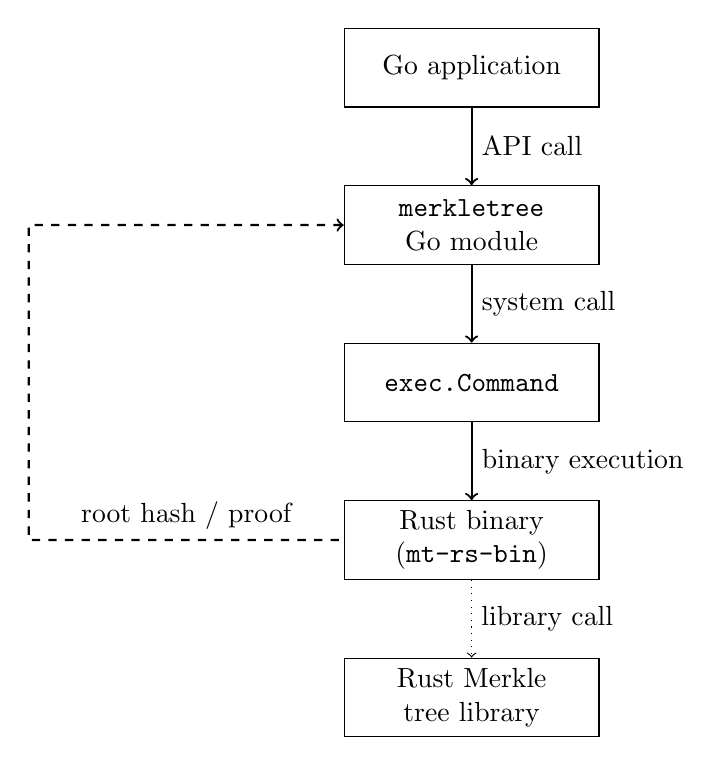
\begin{tikzpicture}[
        node distance=2cm,
    ]

    \tikzstyle{box} = [rectangle, minimum width=3cm, minimum height=1cm,
                       text centered, text width=3cm, draw=black]
    % Nodes
    \node[box] (goapp) {Go application};
    \node[box, below of=goapp] (gomodule) {\texttt{merkletree} Go module};
    \node[box, below of=gomodule] (exec) {\texttt{exec.Command}};
    \node[box, below of=exec] (rustbin) {Rust binary (\texttt{mt-rs-bin})};
    \node[box, below of=rustbin] (rustlib) {Rust Merkle tree library};

    % Arrows
    \draw[->, thick] (goapp) -- (gomodule) node[midway, right] {API call};
    \draw[->, thick] (gomodule) -- (exec) node[midway, right] {system call};
    \draw[->, thick] (exec) -- (rustbin) node[midway, right] {binary execution};
    \draw[->, dotted] (rustbin) -- (rustlib) node[midway, right] {library call};

    % Return arrows
    \draw[<-, thick, dashed] (gomodule.west) -- ++(-4,0) -- ++(0,-4) -- (rustbin.west)
        node[midway, above, sloped] {root hash / proof};

    \end{tikzpicture}
    \caption{Interaction between Go and Rust components. The Go \texttt{merkletree} 
    module invokes the Rust binary via \texttt{exec.Command}, which delegates 
    computation to the Rust Merkle tree library.}
    \label{fig:go-rust-merkle}
\end{figure}

A partial implementation of this Rust binary is shown in Listing
\ref{code:partial-mt-rs-1}. Depending on the flag \texttt{--file}, the binary constructs a 
Merkle tree either from a set of files or from raw data provided as arguments. For instance, 
after compiling and installing the binary as \texttt{mt-rs-bin}, the command 
\texttt{mt-rs-bin --file ff} computes the Merkle root hash for the folder \texttt{ff}, 
which corresponds to the use case in Listing \ref{code:send-shard-server}. Alternatively, 
aggregating per-agent root hashes allows commands such as 
\texttt{mt-rs-bin hash1-ff hash2-ff hash3-ff} to compute the global root hash for folder 
\texttt{ff}, as required in Listing \ref{code:ack-shard}. In both cases, the binary 
produces only the Merkle root hash as a string, which the Go application captures and stores.  

\begin{listing}[H]
\caption{Partial implementation of the Rust binary for Merkle tree creation}
\label{code:partial-mt-rs-1}
\begin{minted}[linenos,fontsize=\footnotesize]{rust}
let tree = if args.file {
    MerkleTree::from_paths(hasher, args.args)
} else {
    let data: Vec<Vec<u8>> = args.args.into_iter()
                                 .map(|s| s.into_bytes()).collect();
    MerkleTree::new(hasher, data)
};

println!("{}", tree.root().hash());
\end{minted}
\end{listing}

The binary can be extended with additional modes, such as proof verification. 
In this case, passing a \texttt{--proof} flag triggers Merkle proof validation instead of 
tree creation, as shown in Listing \ref{code:partial-mt-rs-2}. The output in this case is 
a boolean value (\texttt{true} or \texttt{false}) indicating whether the proof is valid.  

\begin{listing}[H]
\caption{Extension of the Rust binary for Merkle proof verification}
\label{code:partial-mt-rs-2}
\begin{minted}[linenos,fontsize=\footnotesize]{rust}
if let Some(root_hash) = args.proof {
    let nodes = // Build nodes from folders or raw data ...
    let first_node = nodes[0].clone();
    let proofer = DefaultProofer::new(hasher, nodes);
    let proof = proofer.generate(0).expect("Couldn't generate proof");
    let verified = proofer.verify_hash(
                        &proof, first_node.hash().to_string(), &root_hash[..]
                   );
    println!("{}", verified);
} else {
    // Merkle tree creation...
}
\end{minted}
\end{listing}

For completeness, the Go module \texttt{merkletree} provides simplified prototypes for 
proof verification and root computation, listed in \ref{code:prototypes-merkletree-module}. 
These are thin wrappers that internally call the Rust binary via 
\texttt{exec.Command} and capture its output. This design avoids the need for 
complex Go-Rust bindings, while taking advantage of the high-performance Rust 
implementation of the Merkle tree library. In this way, the performance-critical 
logic remains in Rust, whereas the Go application retains a clean and simple 
interface for Merkle tree operations.  

\begin{listing}[htp]
\caption{Prototypes of the \texttt{merkletree} Go module}
\label{code:prototypes-merkletree-module}
\begin{minted}[linenos,fontsize=\footnotesize]{go}
// Verify a Merkle tree proof for some `hashes` with a `rootHash`.
func Verify(hashes [][]byte, rootHash []byte) bool { ... }

// Returns the root hash of the Merkle tree generated for a folder in `path`
func FolderRootHash(path string) ([]byte, error) { ... }

// Returns the root hash of the Merkle tree generated for a list of data
func RootHash(data [][]byte) ([]byte, error) { ... }
\end{minted}
\end{listing}

\paragraph{Signal corruptions}

Finally, this paragraph illustrates how the leader signals corruption for a folder
to the other agents in the Raft cluster. In Listing
\ref{code:command-struct-for-raft}, the reader has already seen the command code
\texttt{SignalCorruption}, which is used here as the operation code. The
associated action is defined by a folder name (top-level or second-level) and a
boolean \texttt{CorruptionStatus} flag.

When the Corruption Check phase (Section \ref{sec:check-corruption}) is triggered,
the leader follows the sequence shown in Figure
\ref{fig:sequence-diagram-check-corruptions}, while also respecting the flow for
handling offline agents as illustrated in Figure
\ref{fig:flow-chart-check-corruption}.

A partial implementation of this flow is presented in Listing
\ref{code:check-corruption-algorithm}. The maps \texttt{hashes1} and
\texttt{hashes2} store folder names as keys and per-agent hashes as values, and
can be used as a backup if some agents are offline. If the first retrieved
\texttt{data} for a top-level folder does not verify against its Merkle proof,
the algorithm iteratively checks each second-level folder nested within it. The
function \texttt{merkletree.IsPathCorrupted} builds a Merkle proof from the
provided \texttt{data} and compares the computed root hash with the reference
root. Internally, it invokes the \texttt{mt-rs-bin} binary, as explained in the
previous paragraph.

Consistency is ensured by Raft: the function \texttt{saveCorruptionState} updates
a global \texttt{corruptions} map that associates each folder (independently of
its level) with a boolean value. Since every update is persisted in the Raft
log, each node in the cluster can rebuild the map locally and remain synchronized
with the cluster state.

\begin{listing}[H]
\caption{Partial implementation of the corruption check algorithm. The leader
verifies Merkle proofs at both top-level and second-level folders, and signals corruption states through the Raft log.}
\label{code:check-corruption-algorithm}
\begin{minted}[linenos,fontsize=\footnotesize]{go}
for folder1, agentHashes1 := range hashes1 {
    root1 := roots1[folder1]
    data := // Retrieve roots for folder1 using agentHashes1 (backup if needed)
    isCorrupted := merkletree.IsPathCorrupted(data, root1)

    if isCorrupted {
        for folder2, agentHashes2 := range hashes2 {
            if strings.HasPrefix(folder2, folder1) {
                root2 := roots2[folder2]
                data := // Retrieve roots for folder2 using agentHashes2
                isCorruptedLevel2 := merkletree.IsPathCorrupted(data, root2)

                if isCorruptedLevel2 {
                    saveCorruptionState(s.RaftServer, folder2, true)
                } else if corruptions[folder2] {
                    // Folder no longer corrupted, but other subfolders may be.
                    saveCorruptionState(s.RaftServer, folder2, false)
                }
            }
        }
        saveCorruptionState(s.RaftServer, folder1, true)
    } else if corruptions[folder1] {
        // Update corruption status for the top-level folder
        // and its second-level children.
    }
}
\end{minted}
\end{listing}

\section{Tests Environment}

The previous section described how the system has been implemented to test every
component following a flow, from the uplodas by an user to the corruption check
from the leader agent in the Raft cluster.

In this new section the reader will read how the tests environment was
setted up with different scenarios, and later will be aware about the obtained
results.

The tests has been completed in a cluster of 9 machines with Ubuntu 24.04.01 LTS (GNU/Linux 6.8.0-51-generic x86_64)

\begin{table}[h!]
    \centering
    \begin{tabular}{|l|c|c|c|}
    \hline
       \textbf{Node ID} & \textbf{IPv4} & \textbf{CPU(s)} & \textbf{Thread(s) per core} &
       \textbf{Core(s) per socket} & \textbf{RAM} & \textbf{Disk} \\
       \hline
        GW & 51.15.221.121 & 8 & 1 & 8 & 32 GB & 45 GB \\

        Agent 1 & 212.47.241.22 & 4 & 1 & 4 & 16 GB & 45 GB \\
        Agent 2 & 51.15.138.169 & 4 & 1 & 4 & 16 GB & 45 GB \\
        Agent 3 & 51.159.178.75 & 4 & 1 & 4 & 8 GB & 45 GB \\
        Agent 4 & 51.158.75.32 & 4 & 1 & 4 & 8 GB & 45 GB \\
        Agent 5 & 51.158.233.202 & 4 & 1 & 4 & 8 GB & 45 GB \\
        Agent 6 & 51.15.108.2 & 4 & 1 & 4 & 8 GB & 45 GB \\
        Agent 7 & 151.115.42.176 & 4 & 1 & 4 & 8 GB & 45 GB \\
        Agent 8 & 151.115.104.48 & 4 & 1 & 4 & 8 GB & 45 GB \\
        \hline
    \end{tabular}
    \caption{...}
    \label{tab:test-vms-specs}
\end{table}


